% skyrius apie chemiją

\section{YAG reakcijos matematinis modeliavimas}

\subsection{YAG sintezė}

\acs{yag} milteliai gali būti sintezuojami keleta skirtingų būdų: Zolis-Gelis procesu, nusodinimu, solvoterminiu procesu, terminio purškimo procesu bei kietafaze reakcija, kuri lieka viena dažniausiai taikomų dėl savo paprastumo bei galimybės pritaikyti masinei gamybai \cite{zhangNovelSynthesisYAG2005}.

\subsection{Kietafazė reakcija}

Šiame darbe yra modeliuojama paskutinė kietafazės reakcijos stadija, kurios metu reaguodami itrio ir aliuminio oksidai sudaro itrio aliuminio granato kristalus arba tiesiog \acs{yag}:
\begin{align*}
  \ce{3Y_2O_3 + 5Al_2O_3 -> 2Y_3Al_5O_12}
\end{align*}

Prieš pradedant reakciją metalų oksidai yra sutrinami iki smulkiagrūdžių miltelių. Metalų oksidų mišinys yra nuolat kaitinamas 1600\degree C laipsnių temperatūroje ir periodiškai maišomas. Eksperimentiniu būdu išmatuota,kad individualių dalelių turiai prie 1600\degree C temperatūros siekia apie $\sqrt{10}\mu\text{m}^3$ \cite{ivanauskasComputationalModellingYAG2009}.

\begin{figure}[h]
  \centering
  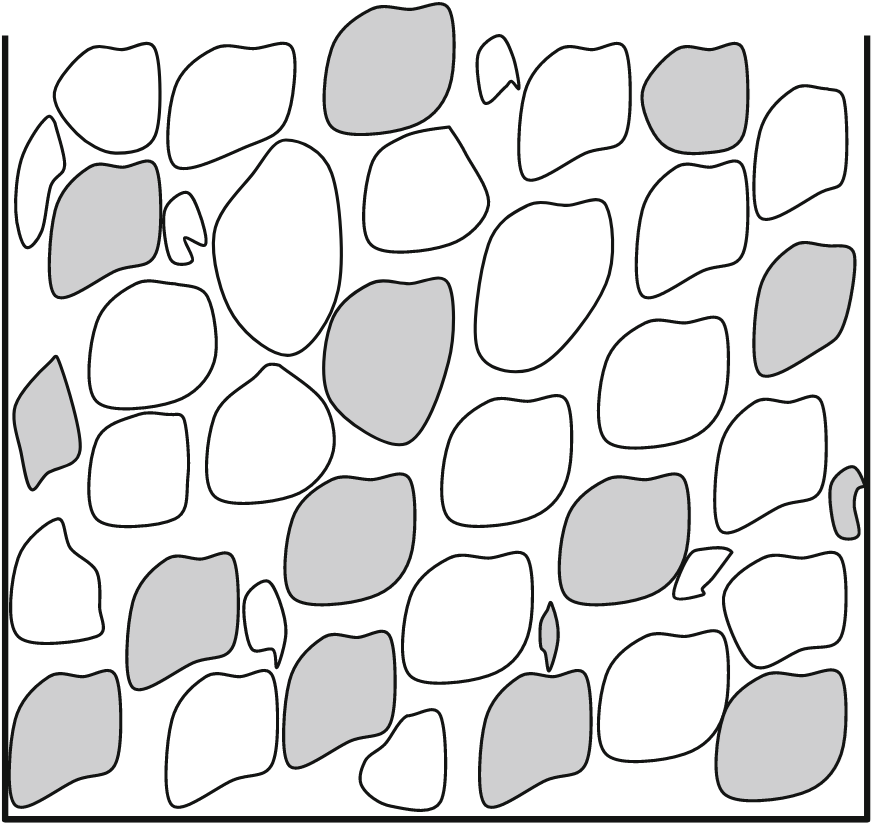
\includegraphics[width=0.25\linewidth]{assets/metal_oxides_mixture.png}
  \label{fig:metal-oxides-mixuter}
  \caption{Priartinto metalų oksidų mišinio iliustracija \cite{}}
\end{figure}

Modeliavimo 

Tokioje temperatūroje metalų oksidai lydosi ir vyksta difuzija, dėl šios priežasties cheminei reakcija yra modeliuojama su difuzijos-reakcijos sistema.
